\documentclass[a4paper, 11pt, notitlepage, english]{article}

\usepackage{babel}
\usepackage[utf8]{inputenc}
\usepackage[T1]{fontenc, url}
\usepackage{textcomp}
\usepackage{amsmath, amssymb}
\usepackage{amsbsy, amsfonts}
\usepackage{graphicx, color, xcolor}
\usepackage{verbatim, listings, fancyvrb}
\usepackage{parskip}
\usepackage{framed}
\usepackage{amsmath}
\usepackage{multicol}
\usepackage{url}
\usepackage{flafter}
\usepackage{simplewick}
\usepackage{amsthm}
\usepackage{bbold}


\usepackage{caption}
\DeclareCaptionLabelSeparator{colon}{. }
\renewcommand{\captionfont}{\small\sffamily}
\renewcommand{\captionlabelfont}{\bf\sffamily}
\usepackage{float}
%\floatstyle{ruled}
%\restylefloat{figure}
\setlength{\captionmargin}{20pt}
%\addto\captionsenglish{\renewcommand{\figurename}{Fig.}}
\usepackage{bigstrut}
\setlength{\tabcolsep}{12pt}


\newtheorem{theorem}[]{Wick's Theorem}[]

\DeclareUnicodeCharacter{00A0}{~}

\definecolor{javared}{rgb}{0.6,0,0} % for strings
\definecolor{javagreen}{rgb}{0.25,0.5,0.35} % comments
\definecolor{javapurple}{rgb}{0.5,0,0.35} % keywords
\definecolor{javadocblue}{rgb}{0.25,0.35,0.75} % javadoc

\lstset{language=python,
basicstyle=\ttfamily\scriptsize,
keywordstyle=\color{javapurple},%\bfseries,
stringstyle=\color{javared},
commentstyle=\color{javagreen},
morecomment=[s][\color{javadocblue}]{/**}{*/},
morekeywords={super, with},
% numbers=left,
% numberstyle=\tiny\color{black},
stepnumber=2,
numbersep=10pt,
tabsize=2,
showspaces=false,
captionpos=b,
showstringspaces=false,
frame= single,
breaklines=true}

\usepackage{geometry}
\geometry{headheight=0.01mm}
\geometry{top=20mm, bottom=20mm, left=34mm, right=34mm}

\renewcommand{\arraystretch}{2}
\setlength{\tabcolsep}{10pt}
\makeatletter
\renewcommand*\env@matrix[1][*\c@MaxMatrixCols c]{%
  \hskip -\arraycolsep
  \let\@ifnextchar\new@ifnextchar
  \array{#1}}
%
% Definering av egne kommandoer og miljøer
%
\newcommand{\dd}[1]{\ \text{d}#1}
\newcommand{\f}[2]{\frac{#1}{#2}} 
\newcommand{\beq}{\begin{equation}}
\newcommand{\eeq}{\end{equation}}
\newcommand{\bra}[1]{\langle #1|}
\newcommand{\ket}[1]{|#1 \rangle}
\newcommand{\braket}[2]{\langle #1 | #2 \rangle}
\newcommand{\brakket}[2]{\langle #1 || #2 \rangle}
\newcommand{\braup}[1]{\langle #1 \left|\uparrow\rangle\right.}
\newcommand{\bradown}[1]{\langle #1 \left|\downarrow\rangle\right.}
\newcommand{\av}[1]{\left| #1 \right|}
\newcommand{\op}[1]{\hat{#1}}
\newcommand{\braopket}[3]{\langle #1 | {#2} | #3 \rangle}
\newcommand{\ketbra}[2]{\ket{#1}\bra{#2}}
\newcommand{\pp}[1]{\frac{\partial}{\partial #1}}
\newcommand{\ppn}[1]{\frac{\partial^2}{\partial #1^2}}
\newcommand{\up}{\left|\uparrow\rangle\right.}
\newcommand{\upup}{\left|\uparrow\uparrow\rangle\right.}
\newcommand{\down}{\left|\downarrow\rangle\right.}
\newcommand{\downdown}{\left|\downarrow\downarrow\rangle\right.}
\newcommand{\updown}{\left|\uparrow\downarrow\rangle\right.}
\newcommand{\downup}{\left|\downarrow\uparrow\rangle\right.}
\newcommand{\bupup}{\left.\langle\uparrow\uparrow\right|}
\newcommand{\bdowndown}{\left.\langle\downarrow\downarrow\right|}
\newcommand{\bupdown}{\left.\langle\uparrow\downarrow\right|}
\newcommand{\bdownup}{\left.\langle\downarrow\uparrow\right|}
\renewcommand{\d}{{\rm d}}
\newcommand{\Res}[2]{{\rm Res}(#1;#2)}
\newcommand{\To}{\quad\Rightarrow\quad}
\newcommand{\eps}{\epsilon}
\newcommand{\inner}[2]{\langle #1 , #2 \rangle}
\renewcommand{\u}{\uparrow}
\renewcommand{\d}{\downarrow}
\newcommand{\dddd}{\d\d\d\d}
\newcommand{\uddd}{\u\d\d\d}
\newcommand{\dudd}{\d\u\d\d}
\newcommand{\ddud}{\d\d\u\d}
\newcommand{\dddu}{\d\d\d\u}
\newcommand{\uudd}{\u\u\d\d}
\newcommand{\udud}{\u\d\u\d}
\newcommand{\uddu}{\u\d\d\u}
\newcommand{\duud}{\d\u\u\d}
\newcommand{\dudu}{\d\u\d\u}
\newcommand{\dduu}{\d\d\u\u}
\newcommand{\uuud}{\u\u\u\d}
\newcommand{\uudu}{\u\u\d\u}
\newcommand{\uduu}{\u\d\u\u}
\newcommand{\duuu}{\d\u\u\u}
\newcommand{\uuuu}{\u\u\u\u}
\newcommand{\m}{\text{-}}
\newcommand{\ui}{{\u_1}}
\newcommand{\uii}{{\u_2}}
\newcommand{\uiii}{{\u_3}}
\newcommand{\di}{{\d_1}}
\newcommand{\dii}{{\d_2}}
\newcommand{\diii}{{\d_3}}

\newenvironment{psmallmatrix}
  {\left(\begin{smallmatrix}}
  {\end{smallmatrix}\right)}

\newenvironment{bsmallmatrix}
  {\left[\begin{smallmatrix}}
  {\end{smallmatrix}\right]}



\newcommand{\bt}[1]{\boldsymbol{#1}}
\newcommand{\mat}[1]{\textsf{\textbf{#1}}}
\newcommand{\I}{\boldsymbol{\mathcal{I}}}
\newcommand{\p}{\partial}
%
% Navn og tittel
%
\author{Jonas van den Brink \\ \texttt{j.v.brink@fys.uio.no}}
\title{Second Midterm Project \\ FYS-KJM4480}

\begin{document}
\maketitle

\vspace{4cm}

\section*{Introduction}

In this project we set up a very simple quantum mechanical system with four particles. We define four spin-degenerate energy-levels the particles can inhabit and force the particles to stay together in pairs, so that effectively two of the four energy-levels will be occupied. We let the energy-levels have a constant spacing in energy, and also define a constant interaction between pairs of particles in the different energy levels.

This system is now fairly simple, letting us calculate the exact ground state energy of the system using full configuration interaction (FCI), something which we normally cannot do. After having found the exact result, we turn to an incomple configuration interaction (CI) approach and study the error we perform in this approximative method. Next we turn to Hartree-Fock formalism, and find the Slater determinant of the system with the lowest possible energy---the reference energy of the system. As we have both the exact energy and the reference energy of the system, we now know the correlation energy. 

Lastly we turn to many-body perturbation theory (MBPT) to look at approximations to the correlation energy. From our previous calculations we then have knowledge of the correlation energy, so we can study how big the error in our approximation is as we increase the order of the perturbation.

In short the goal of this project is to define a system that is so simple that any computations are almost trivial. We do this in the hopes that it will make our various many-body methods more transparant, as well as making it easier for us to compare them with each other.

\clearpage

\subsection*{Exercise 1)}

We start of by defining the following operators
\begin{align*}
  \op{H}_0 &:= \xi \sum_{p \sigma} (p-1)a_{p\sigma}^\dagger a_{p\sigma}, \\
  \op{V} &:= -\frac{1}{2}g \sum_{p q} a_{p+}^\dagger a_{p-}^\dagger a_{q-} a_{q+}, \\
  \op{S}_z &:= \frac{1}{2}\sum_{p\sigma} \sigma a_{p\sigma}^\dagger a_{p\sigma}, \\
  \op{S}^2 &:= \op{S}_z^2 + \frac{1}{2}\big(\op{S}_+\op{S}_- + \op{S}_-\op{S}_+\big), \\
  \op{S}_\pm &:= \sum_p a_{p\pm}^\dagger a_{p\mp}.
\end{align*}
Here, the first operator is our one-body operator and the second is our two-body operator---together these form the Hamiltonian of our system. The final three operators are the standard spin-projection operators. We will start of by showing that our Hamiltonian commutes with the spin projection operators, this result is important as it let's us block-diagonalize the Hamiltonian and look only at unbroken pairs of particles, which will make our further calculations much simpler.

Note that the constants $\xi$ and $g$ chooses the strength of the one-body and the two-body operator we are looking at. Now, as our system does not reflect any real physical system we aren't really interested in scaling our entire system, so the only important factor is the ratio between the strengths of the single-particle operator and the interaction: $\xi/g$. We can then set $\xi=1$ and vary only $g$ without any loss in generality.

To show that the various operators commute, we will use the anti-commutation relations of the standard creation and annihilation operators
$$\{\op{a}_\alpha^\dagger, \op{a}_\beta^\dagger \} = \{\op{a}_\alpha, \op{a}_\beta \} = 0, \qquad \{\op{a}_\alpha^\dagger, \op{a}_\beta \} = \delta_{\alpha\beta},$$

\subsubsection*{The commutator $[\op{H_0}, \op{S}_z]$}
We start by inserting the operators in the definition
\begin{align*}
[\op{H}_0, \op{S}_z] &= \op{H}_0\op{S}_z - \op{S}_z\op{H}_0 \\
&= \frac{1}{2}\sum_{pq \sigma\lambda} \lambda(p-1)\bigg(a_{p\sigma}^\dagger a_{p\sigma}  a_{q\lambda}^\dagger a_{q\lambda}
-   a_{q\lambda}^\dagger a_{q\lambda}  a_{p\sigma}^\dagger a_{p\sigma}\bigg).
\end{align*}
We now swap the two middle operators in the second term, this gives a delta-term
\begin{align*}
[\op{H}_0, \op{S}_z] &= \frac{1}{2}\sum_{pq \sigma\lambda} \lambda(p-1)\bigg(a_{p\sigma}^\dagger a_{p\sigma}  a_{q\lambda}^\dagger a_{q\lambda} 
-   a_{q\lambda}^\dagger \big(\delta_{pq}\delta_{\sigma\lambda} - a_{p\sigma}^\dagger a_{q\lambda} \big) a_{p\sigma}\bigg) \\
&= \frac{1}{2}\sum_{pq \sigma\lambda} \lambda(p-1)\bigg(a_{p\sigma}^\dagger a_{p\sigma}  a_{q\lambda}^\dagger a_{q\lambda}
+   a_{q\lambda}^\dagger a_{p\sigma}^\dagger a_{q\lambda} a_{p\sigma} - \delta_{pq}\delta_{\sigma\lambda}a_{q\lambda}^\dagger a_{p\sigma}
\bigg).
\end{align*}
We now swap the first and second, and third and fourth operator in the second term. We get no delta-terms, and we have no total change in sign
\begin{align*}
[\op{H}_0, \op{S}_z]  &= \frac{1}{2}\sum_{pq \sigma\lambda} \lambda(p-1)\bigg(a_{p\sigma}^\dagger a_{p\sigma}  a_{q\lambda}^\dagger a_{q\lambda}
+   a_{p\sigma}^\dagger  a_{q\lambda}^\dagger  a_{p\sigma} a_{q\lambda} - \delta_{pq}\delta_{\sigma\lambda}a_{q\lambda}^\dagger a_{p\sigma}
\bigg).
\end{align*}
Again we swap the two middle operators, getting another delta term
\begin{align*}
 [\op{H}_0, \op{S}_z]  &= \frac{1}{2}\sum_{pq \sigma\lambda} \lambda(p-1)\bigg(a_{p\sigma}^\dagger a_{p\sigma}  a_{q\lambda}^\dagger a_{q\lambda}
+  a_{p\sigma}^\dagger  \big(\delta_{pq}\delta_{\lambda\sigma} - a_{p\sigma} a_{q\lambda}^\dagger  \big) a_{q\lambda} - \delta_{pq}\delta_{\sigma\lambda}a_{q\lambda}^\dagger a_{p\sigma}
\bigg) \\
&= \frac{1}{2}\sum_{pq \sigma\lambda} \lambda(p-1) \delta_{pq}\delta_{\lambda\sigma}\big(a_{p\sigma}^\dagger a_{q\lambda} - a_{q\lambda}^\dagger a_{p\sigma}
\big).
\end{align*}
Due to the Kronecker-deltas the only surviving terms in the sums will have $p=q$ and $\sigma=\lambda$, meaning the two terms will cancel out, so we have
\begin{align*}
 [\op{H}_0, \op{S}_z] &= 0,
\end{align*}
and we have confirmed that $\op{H}_0$ and $\op{S}_z$ commute.

\subsubsection*{The commutator $[\op{V}, \op{S}_z]$}
Again, we start from the definition
\begin{align*}
[\op{V}, \op{S}_z] &= \op{V}\op{S}_z - \op{S}_z\op{V} \\
&= \frac{g}{4}\sum_{pqr\sigma} \sigma \bigg(a_{r\sigma}^\dagger a_{r\sigma} a_{p+}^\dagger a_{p-}^\dagger a_{q-} a_{q+} - a_{p+}^\dagger a_{p-}^\dagger a_{q-} a_{q+} a_{r\sigma}^\dagger a_{r\sigma} \bigg).
\end{align*}
We now move the $a_{r\sigma}^\dagger$-operator in the second term to the front by succesively swapping it to the left
\begin{align*}
a_{p+}^\dagger a_{p-}^\dagger &a_{q-} a_{q+} a_{r\sigma}^\dagger a_{r\sigma} \\ 
&= a_{p+}^\dagger a_{p-}^\dagger a_{q-} \big(\delta_{qr}\delta_{\sigma+} -  a_{r\sigma}^\dagger a_{q+} \big) a_{r\sigma} \\
&=\delta_{qr}\delta_{\sigma+} a_{p+}^\dagger a_{p-}^\dagger a_{q-} a_{r\sigma}  - a_{p+}^\dagger a_{p-}^\dagger \big(\delta_{qr}\delta_{\sigma-} -  a_{r\sigma}^\dagger a_{q-} \big) a_{q+} a_{r\sigma} \\
&=\delta_{qr}\delta_{\sigma+} a_{p+}^\dagger a_{p-}^\dagger a_{q-} a_{r\sigma}  - \delta_{qr}\delta_{\sigma-} a_{p+}^\dagger a_{p-}^\dagger a_{q+} a_{r\sigma} +  a_{r\sigma}^\dagger  a_{p+}^\dagger a_{p-}^\dagger a_{q-}  a_{q+} a_{r\sigma}.
\end{align*}
In the final term here, we now move the $a_{r\sigma}$ by successive shifts
\begin{align*}
a_{r\sigma}^\dagger  a_{p+}^\dagger & a_{p-}^\dagger a_{q-}  a_{q+} a_{r\sigma} \\
&= a_{r\sigma}^\dagger  a_{p+}^\dagger \big(\delta_{pr} \delta_{\sigma -} -  a_{r\sigma} a_{p-}^\dagger\big) a_{q-}  a_{q+} \\
&= \delta_{pr} \delta_{\sigma -} a_{r\sigma}^\dagger  a_{p+}^\dagger a_{q-}  a_{q+} -  a_{r\sigma}^\dagger  \big(\delta_{pr}\delta_{\sigma+} - a_{r\sigma}a_{p+}^\dagger\big) a_{p-}^\dagger a_{q-}  a_{q+} \\
&= \delta_{pr} \delta_{\sigma -} a_{r\sigma}^\dagger  a_{p+}^\dagger a_{q-}  a_{q+} -  \delta_{pr}\delta_{\sigma+} a_{r\sigma}^\dagger  a_{p-}^\dagger a_{q-}  a_{q+} + a_{r\sigma}^\dagger a_{r\sigma}a_{p+}^\dagger a_{p-}^\dagger a_{q-}  a_{q+}.\\
\end{align*}
Putting this result back into the original expression gives
\begin{align*}
[\op{V}, \op{S}_z] = \frac{g}{4}\sum_{pqr\sigma} \sigma \big(&
\delta_{pr}\delta_{\sigma+} a_{r\sigma}^\dagger  a_{p-}^\dagger a_{q-}  a_{q+}
+ \delta_{qr}\delta_{\sigma-} a_{p+}^\dagger a_{p-}^\dagger a_{q+} a_{r\sigma}\\[-0.3cm]
&\qquad- \delta_{qr}\delta_{\sigma+} a_{p+}^\dagger a_{p-}^\dagger a_{q-} a_{r\sigma}  
- \delta_{pr} \delta_{\sigma -} a_{r\sigma}^\dagger  a_{p+}^\dagger a_{q-}  a_{q+} \big).
\end{align*}
We now perform the sum over $\sigma$, giving
\begin{align*}
[\op{V}, \op{S}_z] = \frac{g}{4}\sum_{pqr} &
\delta_{pr} \big(a_{r+}^\dagger  a_{p-}^\dagger a_{q-}  a_{q+} + a_{r-}^\dagger a_{p+}^\dagger a_{q-}  a_{q+} \big) \\[-0.3cm]
&\qquad - \delta_{qr} \big( a_{p+}^\dagger a_{p-}^\dagger a_{q+} a_{r-} + a_{p+}^\dagger a_{p-}^\dagger a_{q-} a_{r+} \big).
\end{align*}
We now perform the sum over $p$ and $q$, we see the only surviving terms are those were $p=r$ or $q=r$, giving
\begin{align*}
[\op{V}, \op{S}_z] = \frac{g}{4}\sum_{r} \big(
a_{r+}^\dagger  a_{r-}^\dagger a_{r-}  a_{r+} + a_{r-}^\dagger a_{r+}^\dagger a_{r-}  a_{r+}  -  a_{r+}^\dagger a_{r-}^\dagger a_{r+} a_{r-} - a_{r+}^\dagger a_{r-}^\dagger a_{r-} a_{r+} \big).
\end{align*}
We see that the terms cancel each other out, leaving
\begin{align*}
 [\op{V}, \op{S}_z] &= 0,
\end{align*}
and we have confirmed that $\op{V}$ and $\op{S}_z$ commute.

\subsubsection*{The commutator $[\op{H_0}, \op{S}_\pm]$}
From the definition, we have
\begin{align*}
[\op{H}_0, \op{S}_\pm] &= \op{H}_0\op{S}_\pm - \op{S}_\pm\op{H}_0 \\
&= 
\xi \sum_{pq \sigma} (p-1) \big( a_{p\sigma}^\dagger a_{p\sigma}  a_{q\pm}^\dagger a_{q\mp}       
- a_{q\pm}^\dagger a_{q\mp} a_{p\sigma}^\dagger a_{p\sigma}\big).
\end{align*}
Again, we shift the operators around in the second term around, so that it cancels with the first term, we get the following result
\begin{align*}
[\op{H}_0, \op{S}_\pm] &= \xi \sum_{pq \sigma} (p-1) \delta_{pq} (\delta_{\sigma \pm} - \delta_{\sigma \mp}).
\end{align*}
We can now take the sum over $\sigma$, which makes the entire commutator vanish, as the two Kronecker-delta's with $\sigma $ cancel each other out, so we have
\begin{align*}
[\op{H}_0, \op{S}_\pm] &= 0.
\end{align*}
And $\op{H}_0$ commutes with $\op{S}_\pm$.


\subsubsection*{The commutator $[\op{V}, \op{S}_\pm]$}
From the definition, we have
\begin{align*}
[\op{V}, \op{S}_\pm] &= \op{V}\op{S}_\pm - \op{S}_\pm\op{V} \\
&= -\frac{g}{2}\sum_{pqr} a_{p+}^\dagger a_{p-}^\dagger a_{q-} a_{q+} a_{r\pm}^\dagger a_{r\mp} - a_{r\pm}^\dagger a_{r\mp} a_{p+}^\dagger a_{p-}^\dagger a_{q-} a_{q+}.
\end{align*}
Shifting the operators around in the second term makes it cancel with the first, but shifting the operators generates some terms, we have
\begin{align*}
[\op{V}, \op{S}_\pm] &= \frac{g}{2}\sum_{pqr}
\big(\delta_{pr}\delta_{\mp +}  a_{r\pm}^\dagger a_{p-}^\dagger a_{q-} a_{q+}
- \delta_{pr}\delta_{\mp -} a_{r\pm}^\dagger a_{p+}^\dagger a_{q-} a_{q+} \\[-0.2cm]
&\qquad\qquad\qquad + \delta_{qr}\delta_{\pm -} a_{p+}^\dagger   a_{p-}^\dagger a_{q+} a_{r\mp}
- \delta_{qr} \delta_{\pm +}a_{p+}^\dagger   a_{p-}^\dagger a_{q-} a_{r\mp}\big).
\end{align*}
Summing over $p$ and $q$ gives
\begin{align*}
[\op{V}, \op{S}_\pm] &= \frac{g}{2}\sum_{r}
\big(\delta_{\mp +} a_{r\pm}^\dagger a_{r-}^\dagger a_{r-} a_{r+}
- \delta_{\mp -} a_{r\pm}^\dagger a_{r+}^\dagger a_{r-} a_{r+} \\[-0.2cm]
&\qquad\qquad\qquad + \delta_{\pm -} a_{r+}^\dagger   a_{r-}^\dagger a_{r+} a_{r\mp}
-  \delta_{\pm +}a_{r+}^\dagger   a_{r-}^\dagger a_{r-} a_{r\mp}\big).
\end{align*}
We now see that for both $\op{S}_+$ and $\op{S}_-$ there is a chain of two equal creation or annihilation operators, which kill any state, so we have
\begin{align*}
[\op{V}, \op{S}_\pm] &= 0.
\end{align*}


\subsubsection*{The commutator $[\op{H}_0, \op{S}^2]$}

To compute the commutator between $\op{H}_0$ and $\op{S}^2$ we express the total spin by the operators $\op{S}_z$ and $\op{S}_\pm$, so we get
\begin{align*}
[\op{H}_0, \op{S}^2] &= [\op{H}_0, \op{S}_z^2 + \frac{1}{2}\big(\op{S}_+\op{S}_- + \op{S}_-\op{S}_+\big)] \\
&= [\op{H}_0, \op{S}_z^2] + \frac{1}{2}[\op{H}_0, \op{S}_+\op{S}_-] + \frac{1}{2}[\op{H}_0, \op{S}_-\op{S}_+].
\end{align*}
We now use that fact that for any operators $\op{A}$, $\op{B}$ and $\op{C}$
\begin{align*}
[\op{A},\op{B}\op{C}] = \op{A}\op{B}\op{C} - \op{B}\op{C}\op{A} = \op{A}\op{B}\op{C} - \op{B}\op{A}\op{C} + \op{B}\op{A}\op{C} - \op{B}\op{C}\op{A} = [\op{A},\op{B}]\op{C} + \op{B}[\op{A},\op{C}].
\end{align*}
So we get
\begin{align*}
[\op{H}_0, \op{S}_z^2] &= [\op{H}_0, \op{S}_z]\op{S}_z + \op{S}_z[\op{H}_0, \op{S}_z] = 0, \\
[\op{H}_0, \op{S}_+\op{S}_-] &= [\op{H}_0, \op{S}_+]\op{S}_- + \op{S}_+[\op{H}_0, \op{S}_-] = 0, \\
[\op{H}_0, \op{S}_-\op{S}_+] &= [\op{H}_0, \op{S}_-]\op{S}_+ + \op{S}_-[\op{H}_0, \op{S}_+] = 0.
\end{align*}
So we see that 
$$[\op{H}_0, \op{S}^2] = 0.$$

\subsubsection*{The commutator $[\op{V}, \op{S}^2]$}

We immediately see that $\op{V}$ and $\op{S}^2$ commutes from the same argument as for $\op{H}_0$.
$$[\op{V}, \op{S}^2] = 0.$$

\subsection*{Rewriting the Hamiltonian}

We have now seen that our Hamiltonian commutes with all the spin projection operators, this means that the spin of our system is a conserved quantity. We will start of by requiring a total spin of $S=0$, and this will be a conserved quantity. 

As our Hamiltonian will preserve pair of particles, we introduce the \emph{pair creation and annihilation operators}
$$\op{P}_p^+ = a_{p+}^\dagger a_{p-}^\dagger \qquad \op{P}_p^- = a_{p-} a_{p+},$$
which lets us write $\op{V}$ as
$$\op{V} = -\frac{1}{2}g \sum_{pq} \op{P}_p^+ \op{P}_q^-.$$
And our full Hamiltonian becomes
\begin{align*}
	\op{H} = \op{H_0} + \op{V} = \sum_{p \sigma} (p-1)a_{p\sigma}^\dagger a_{p\sigma}-\frac{1}{2}g \sum_{pq} \op{P}_p^+ \op{P}_q^-.
\end{align*}
So we see that our system will always consist of unbroken pairs.

We can easily show that the pair creation and annihilation operators commute with themselves
\begin{align*}
[\op{P}^\pm_p, \op{P}^\pm_q] = a_{p\pm}^\dagger a_{p\mp}^\dagger a_{q\pm}^\dagger a_{q\mp}^\dagger - a_{q\pm}^\dagger a_{q\mp}^\dagger  a_{p\pm}^\dagger a_{p\mp}^\dagger = [\op{P}^\pm_q,\op{P}^\pm_p].
\end{align*}
This result is very intuitive, as changing the order of two pair creation or annihilation operators corresponds to interchanging two pair of fermions, which will give a total change in sign of $(-)^2$, so the commutators should commute instead of anti-commute such as for the single-particle creation and annihilation operators.

\clearpage

\section*{Exercise 2)}

We now look at our system of four particles. As we saw, we require a total spin of $S=0$ and won't have any broken pairs. We also limit our system to only inhabit the four lowest levels $p=1,2,3,4$.  This gives rise to six different Slater determinants
\begin{align*}
	\ket{\Phi^{0}} &= \op{P}_1^+ \op{P}_2^+ \ket{0}, \qquad \ket{\Phi_2^{3}} = \op{P}_1^+ \op{P}_3^+ \ket{0}, \qquad \ket{\Phi_2^{4}} = \op{P}_1^+ \op{P}_4^+ \ket{0}, \\
	\ket{\Phi_1^{3}} &= \op{P}_2^+ \op{P}_3^+ \ket{0}, \qquad \ket{\Phi_1^{4}} = \op{P}_2^+ \op{P}_4^+ \ket{0}, \qquad \ket{\Phi_{12}^{34}} = \op{P}_3^+ \op{P}_4^+ \ket{0}.
\end{align*}
Where we have denoted the first state as our Fermi-vacuum, the four following Slater determinants (SD) are then four 2-particle 2-hole states, and the final SD is a 4-particle 4-hole state. The Slater determinants are illustrated in figure \ref{fig:2}.

\begin{figure}[htpb]
	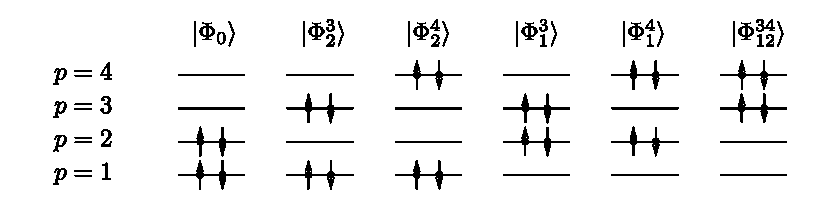
\includegraphics[width=\textwidth]{project2b.pdf}
	\caption{Sketch of the six possible Slater determinants. \label{fig:2}}
\end{figure}

These six Slater determinants are orthonormal and span a six-dimensional Hilbert space. We want to compute the matrix representation of the Hamiltonian in this space, which is given by
$$H_{ij} = \braopket{\Phi_i}{\op{H}}{\Phi_j},$$
where $\{\Phi_i\}_{i=1}^6$ is the set of the six Slater determinants. To calculate the different matrix elements, it's easiest to split up the Hamiltonian, so we have
$$H_{ij} = \braopket{\Phi_i}{\op{H}_0}{\Phi_j} + \braopket{\Phi_i}{\op{V}}{\Phi_j}. $$

The one-body operator is
\begin{align*}
\op{H}_0 = \sum_{p\sigma} (p-1)a_{p\sigma}^\dagger a_{p\sigma},
\end{align*}
so we see that the for the off-diagonal terms, the one-body contribution vanishes. For the diagonal terms we find
\begin{align*}
\braopket{\Phi_0}{\op{H}_0}{\Phi_0} &= 2, \qquad \braopket{\Phi_2^3}{\op{H}_0}{\Phi_2^3} = 4, \qquad \braopket{\Phi_2^{4}}{\op{H}_0}{\Phi_2^{4}} = 6, \\
\braopket{\Phi_1^3}{\op{H}_0}{\Phi_1^{3}} &= 6, \qquad \braopket{\Phi_2^{4}}{\op{H}_0}{\Phi_2^{4}} = 8, \qquad \braopket{\Phi_{12}^{34}}{\op{H}_0}{\Phi_{12}^{34}} = 10.
\end{align*}

For the two-body operator we have
\begin{align*}
\op{V} = -\frac{g}{2}\sum_{pq} P_p^+ P_q^-.
\end{align*}
When calculating the matrix elements, we see that we can either have no non-coincidences, two non-coincidences or four non-coincidences. Another way to state this is to say that there can a mismatch of zero, one or two pairs. 

If there is a mismatch of two pairs, the matrix element clearly vanishes.
\begin{align*}
\braopket{\Phi_0}{\op{V}}{\Phi_{12}^{34}} = 0, \\
\braopket{\Phi_2^3}{\op{V}}{\Phi_{1}^{4}} = 0, \\
\braopket{\Phi_2^4}{\op{V}}{\Phi_{1}^{3}} = 0. \\
\end{align*}

Next, if there is a mismatch of one pair, the two-body operator has to remove it, meaning there is only one term in the sum over $p$ and $q$ that will contribute to the matrix elements, so we have
\begin{align*}
\braopket{\Phi_0}{\op{V}}{\Phi_i^a} = -g/2, \\
\braopket{\Phi_i^a}{\op{V}}{\Phi_i^{b}} = -g/2, \\
\braopket{\Phi_i^a}{\op{V}}{\Phi_j^{a}} = -g/2, \\
\braopket{\Phi_i^a}{\op{V}}{\Phi_{12}^{34}} = -g/2.
\end{align*}
Note that we do not have to worry about a change in sign for the terms due to the commutation relations of the pair creation and annihilation operators.

When there is no mismatches between the pairs, i.e., when looking at the diagonal terms,  there are two terms in the sum that contribute to the matrix elements, so we have
\begin{align*}
\braopket{\Phi_i}{\op{V}}{\Phi_i} = -g.
\end{align*}

We summarize our results by setting up the Hamiltonian matrix
\begin{align*}
\op{H} = \begin{pmatrix}
2 - g &  -g/2 & -g/2  & -g/2  & -g/2  & 0     \\
-g/2  & 4 - g & -g/2  & -g/2  & 0     & -g/2  \\
-g/2  & -g/2  & 6 - g &	0     & -g/2  & -g/2  \\              
-g/2  & -g/2  & 0     & 6 - g &	-g/2  & -g/2  \\                         
-g/2  &	0	  & -g/2  & -g/2  & 8 - g & -g/2  \\
0     &  -g/2 & -g/2  & -g/2  &  -g/2 & 10 - g 
\end{pmatrix}
\end{align*}

Numerically, we find the eigenvalues and eigenvectors of this matrix. The lowest eigenvalue then corresponds to the ground state energy. Numerically, we can generate the Hamiltonian matrix and find the eigenvalue for any value of $g$, effectively giving us the ground state energy as a function of the strength of the interaction. We will for the rest of this project refer to that energy as the ``exact'' energy of the system. The exact energy function is shown in the figure on the following page.

The diagonalization of the Hamiltonian matrix also gives us the coefficients in the exact expansion
$$\ket{\Psi} = C_0\ket{\Phi_0} + C_{2}^{3} \ket{\Phi_{2}^{3}} +  C_{2}^{4} \ket{\Phi_{2}^{4}} +  C_{1}^{3} \ket{\Phi_{1}^{3}} +  C_{1}^{4} \ket{\Phi_{1}^{4}} + C_{12}^{34} \ket{\Phi_{12}^{34}}.$$
Listing these for different strengths of the interaction isn't really interesting, so we will give them only for $g=1/2$ as an example, in that case they are
\begin{align*}
C_0 &= -0.996, \qquad C_2^3 = -0.066, \,\, \qquad C_2^4 = -0.034, \\
C_1^3 &= -0.034, \qquad   C_1^5 = -0.022, \qquad C_{12}^{34} = -0.002.
\end{align*}
Note that it is only the magnitude of a coefficient that is of importance, the sign is not interesting. We see that the ground state is comprised of mainly our reference state $\ket_{0}$, this is of course not very suprising, as this is the SD with clearly the lowest energy in and of itself, as the interaction is a lot weaker than the single-particle operator in this case, we don't expect a hugh contribution from the excited states. We also see that $|C_2^4|^2 = |C_1^3|$, which is also unsurprising, as we see that these two SDs have the same diagonal term in the Hamiltonian, i.e., they represent the exact same energy.



\begin{figure}[htpb]
	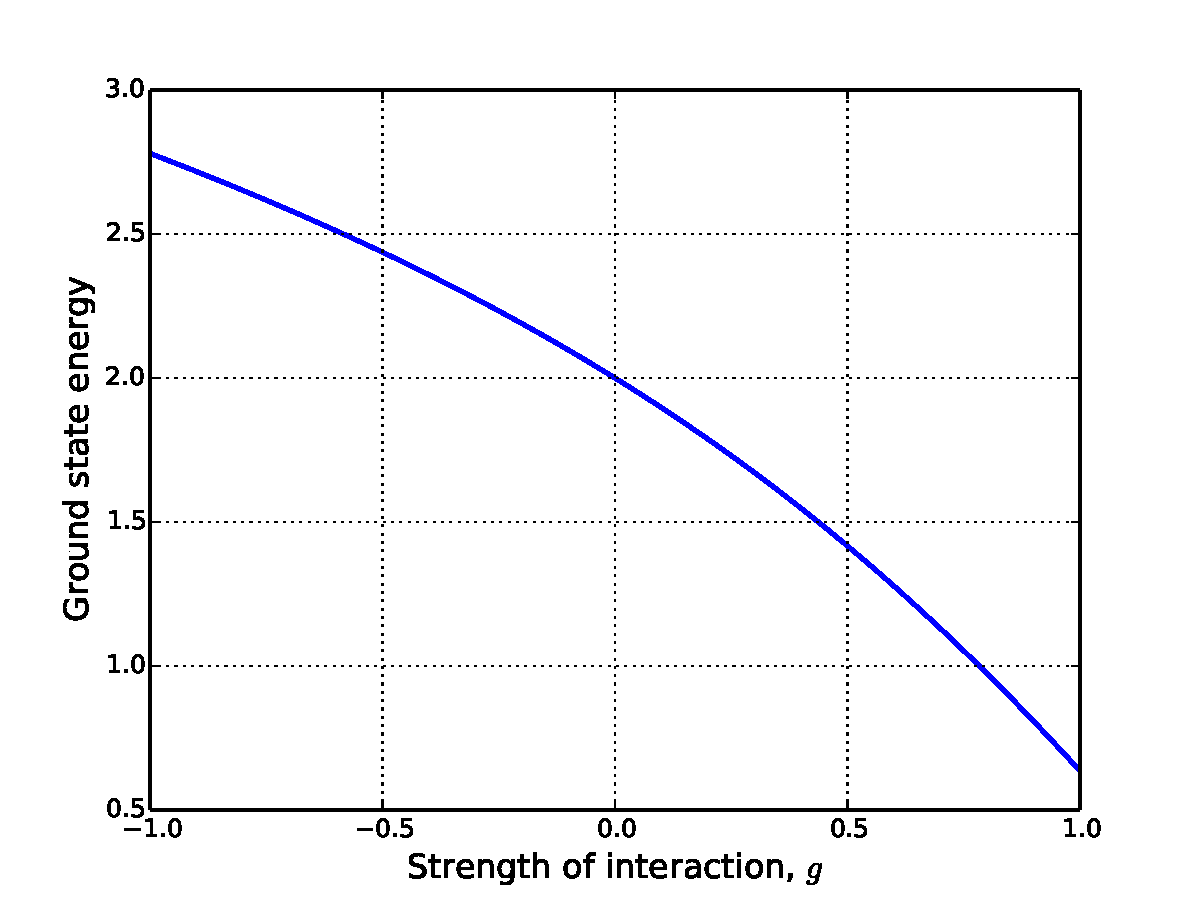
\includegraphics[width=\textwidth]{proj1_exact.pdf}
	\caption{Exact ground state energy as a function of the strength of the interaction. \label{fig:plot1}}
\end{figure}

\clearpage

\section*{Exercise 3)}

We now limit our system to at most two-particle-two-hole excitations, meaning only a single pair of particles can be excited. This means we have to discard $\ket{\Phi_{12}^{34}}$, and only look at a five-dimensional system. We have now effectively turned from full configuration intercation (FCI), an exact method, to a non-full configuration interaction (CI), an approximative method.

The Hamiltonian matrix is unchanged except for the fact that it is reduced to a five-by-five matrix by stripping the rows and columns that corresponded to the removed Slater determinant. The Hamiltonian matrix is
\begin{align*}
\op{H} = \begin{pmatrix}
2 - g &  -g/2 & -g/2  & -g/2  & -g/2  \\
-g/2  & 4 - g & -g/2  & -g/2  & 0     \\
-g/2  & -g/2  & 6 - g &	0     & -g/2  \\              
-g/2  & -g/2  & 0     & 6 - g &	-g/2  \\                         
-g/2  &	0	  & -g/2  & -g/2  & 8 - g \
\end{pmatrix}
\end{align*}

Again we calculate the ground state energy as a function of the interaction strength $g$. The results are shown alongside the exact result in the following figure. As we see from the figure, the approximation is almost spot on, even when the interaction is strong. This is unsurprising. 

\begin{figure}[htpb]
\centering
  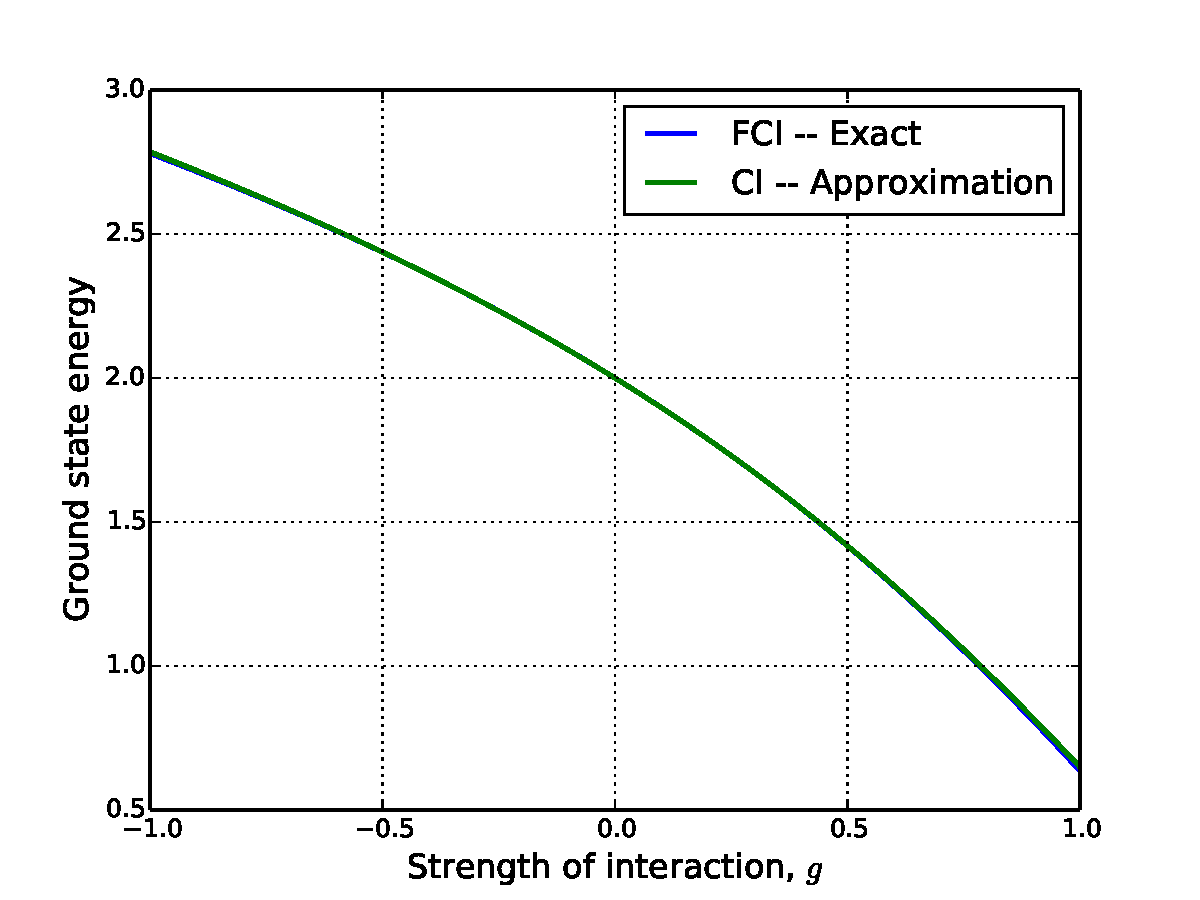
\includegraphics[width=0.88\textwidth]{proj1_approx.pdf}
  \caption{The exact ground state energy as a function of the strength of the interaction, found with FCI and an approximation found with a non-full CI. \label{fig:plot2}}
\end{figure}
In the previous exercise we saw how the ground state was comprised almost entirely of the reference SD, there are also 4 possible 2p2h states, all with lower energies than the excluded 4p4h. Note also that CI is a variational method, which is reflected in the figure as the approximate energy is always slightly above the exact result.

Just like for the FCI case, let us look at the coefficents in the expansion of the ground state at $g=1/2$
\begin{align*}
C_0 &= -0.985, \quad C_2^3 = -0.135,  \quad C_2^4 = -0.071, \quad C_1^3 &= -0.0714, \quad C_1^5 = -0.046.
\end{align*}
So compared to the true ground state of the system, we see that we have less of our reference state and more of all the 2p2h states.

From our results, we now see some important differences between FCI and CI. Full configuration interaction is an exact method, but is only possible if and only if we have a complete and finite SD basis for our system. In practice, we usually \emph{don't} have this. Non-complete CI however, is always possible, but only give approximative results. The method is variational however, so we are always guaranteed that the approximation will be equal or bigger to the true result. Non-complete CI also guarantees that including more excitations will give an unchanged or better result, at least for a given reference state. This is a big difference from perturbation theory, which is not variational and provides no guarantee that including more orders won't give a worse result---we will see this later in this project.

In a FCI case, we are including all possible exictations to infinite order, meaning we have all possible 1p1h SDs, all possible 2p2h SDs and so on. In the CI case, we truncate those excitations somewhere. In our example we limited the excitations to at most 2p2h. We still got the contribution from those 2p2h excitation to infinite order. If we were to draw the diagrams of the interactions that contribute to this CI case, there would be an infinite number of them, as we can have arbitrarily long chains of operators that still only have at most 2p2h intermediate states. 

When we look at perturbation theory Later in this project, we will sum the 2p2h excitations first to second order and third order and finally to fourth order. As we increase the order, there are more contributions to the 2p2h excitations. You can see the 2p2h excitations to second and third order in figure 2 in the exercises, and then to fourth order in figure 4. We will explain how these diagrams are interpret later, when we get to the perturbation part of the project. 

We now end this exercise by showing some examples of 2p2h excitations that build up the CI approximation.

\vspace{0.2cm}

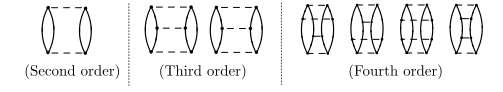
\includegraphics[width=\textwidth]{project2_3}


\clearpage

\section*{Exercise 4)}

We now turn to Hartree-Fock theory. First we will partition our Hamiltonian and define our Fock operator. This will illuminate the difference between a cannonical and a non-cannonical Hartree-Fock case. For each of these cases, as well as a general (i.e., a non Hartree-Fock) case, we will set up the normal-ordered Hamiltonian in both diagramatic and algebraic form.


\subsection*{Partitioning the Hamiltonian}

If we limit ourselves to at most two-body interactions, the Hamiltonian of any system can be generally written as a sum of one-body and two-body operators, which in second quantization looks like
$$\op{H} = \op{H}_1 + \op{H}_2 = \sum_\mu \op{h}_\mu + \sum_{\mu\nu} \op{v}_{\mu\nu}.$$
For our system we have a single one-body and a single two-body interaction, labeling them $\op{h}_0$ and $\op{v}$, we get
$$\op{H} = \sum_{\alpha\beta} \braopket{\alpha}{\op{h}_0}{\beta}\alpha^\dagger \beta + \frac{1}{4}\sum_{\alpha\beta\gamma\delta}\brakket{\alpha\beta}{\gamma\delta}\alpha^\dagger \beta^\dagger \delta \gamma,$$
where we use Shavitt and Bartlet's shorthand of $\brakket{\alpha\beta}{\gamma\delta} = \braopket{\alpha\beta}{\op{v}}{\gamma\delta}_{\rm AS}$.

Using Wick's theorem, we can write these out as 
\begin{align*}
\op{H}_1 &= \sum_{pq}\braopket{p}{\op{h}_0}{q}\{\op{p}^\dag \op{q}\} + \sum_{i}\braopket{i}{\op{h}_0}{i}, \\
\op{H}_2 &= \frac{1}{4}\sum_{pqrs} \brakket{pq}{rs} \{\op{p}^\dag \op{q}^\dag \op{s}\op{r}\} + \sum_{pqi} \brakket{pi}{qi} \{ \op{p}^\dag \op{q} \} + \frac{1}{2}\sum_{ij} \brakket{ij}{ij}.
\end{align*}
We now define the \emph{reference energy} as
$$E_{\rm ref} = \sum_{i}\braopket{i}{\op{h}_0}{i} + \frac{1}{2}\sum_{ij} \brakket{ij}{ij}.$$
Which enables us to split the Hamiltonian into its normal-ordered part and the reference energy
$$\op{H} = \op{H}_{\rm N} + E_{\rm ref}.$$
The normal-ordered Hamiltonian is then
$$\op{H}_{\rm N} = \sum_{pq}\braopket{p}{\op{h}_0}{q}\{\op{p}^\dag \op{q}\}  + \sum_{pqi} \brakket{pi}{qi}\{\op{p}^\dag \op{q}\}  + \frac{1}{4}\sum_{pqrs} \brakket{pq}{rs} \{\op{p}^\dag \op{q}^\dag \op{s}\op{r}\}.$$
We now relabel the first two terms into the normal-ordered \emph{Fock-operator}, giving us
$$\op{H}_{\rm N} = \op{F}_{\rm N} + \frac{1}{4}\sum_{pqrs} \brakket{pq}{rs} \{\op{p}^\dag \op{q}^\dag \op{s}\op{r}\}.$$
We can now think of the normal-ordered Hamiltonian as the sum of a one-body part and the perturbation
$$\op{W}_{\rm N}  =\frac{1}{4}\sum_{pqrs} \brakket{pq}{rs} \{\op{p}^\dag \op{q}^\dag \op{s}\op{r}\},$$
we will get back to this when we turn to many-body perturbation theory.

\clearpage

For now, we will look closer at the normal-ordered Fock-operator
$$\op{F}_{\rm N} = \sum_{pq}\braopket{p}{\op{h}_0}{q}\{\op{p}^\dag \op{q}\}  + \sum_{pqi} \brakket{pi}{qi} \{\op{p}^\dag \op{q}\} = \sum_{pq} f_{pq} \{\op{p}^\dagger \op{q} \},$$
where
$$f_{pq} = \braopket{p}{\op{h}_0}{q} + \sum_{pqi} \brakket{pi}{qi}  = h_{pq} + u_{pq}.$$
We see that the exact form of the Fock-matrix is then the result of the form of the one-body and two-body operators $\op{h}_0$ and $\op{v}$ and also of our choice of single-particle basis. 

The form of the Fock-matrix is quite important for our further discussion of how to solve the problem, and so we will label three different cases:
\begin{enumerate}
	\item First we have the possibility of the Fock-matrix being purely diagonal
	$$f_{pq} = \eps_p \delta_{pq},$$
	this case is known as the \emph{cannonical Hartree-Fock} case.
	\item Next, we have the case where the Fock-matrix is not entirely diagonal, but it is \emph{block-diagonal}, meaning the blocks of the Fock-matrix corresponding to the matrix elements between hole and particle states vanish. So we have
	$$f_{ai} = 0,$$
	this is the \emph{non-cannonical} Hartree-Fock case. Note that some people do not distinguish between the cannonical and non-cannonical HF cases.
	\item All cases not covered by the two HF cases are collectively reffered to as \emph{general} cases.
\end{enumerate}
As the normal-ordered Fock-operator can be non-diagonal, it is often conveniant to split it into its diagonal and off-diagonal contributions
$$\op{F}_{\rm N} = \sum_p f_{pp}\{\op{p}^\dagger \op{p}\} + \sum_{p\neq q} f_{pq}\{\op{p}^\dagger \op{q}\} = \op{F}_{\rm N}^{\rm D} + \op{F}_{\rm N}^{\rm O}.$$
In the cases where $\op{F}_{\rm N}^{\rm O} \neq 0$, it is common to include this part of the Fock-operator in the perturbation.

The total normal-product Hamiltonian is then
$$\op{H}_{\rm N} = \op{F}_{\rm N} + \op{W}_{\rm N} = \op{F}^{\rm d}_{\rm N} + \op{F}^{\rm o}_{\rm N} + \op{W}_{\rm N} = \op{F}^{\rm d}_{\rm N} + \tilde{W}_{\rm N}.$$

\subsubsection*{The Hamiltonian in diagrams}

We will now draw the diagrams representing the Hamiltonian for all three cases. First of, let us draw the the reference energy, which is what separates the complete Hamiltonian from the normal-ordered Hamiltonian.

\begin{centering}

\includegraphics[width=\textwidth]{project2_4a}
\end{centering}

\clearpage

Let us now move on to the normal-ordered Hamiltonian, which is given by
$$\op{H}_{\rm N} = \op{F}_{\rm N} + \op{W}_{\rm N}.$$
For all three cases the $\op{W}_{\rm N}$ term is the same, so let us show that term first

\begin{centering}
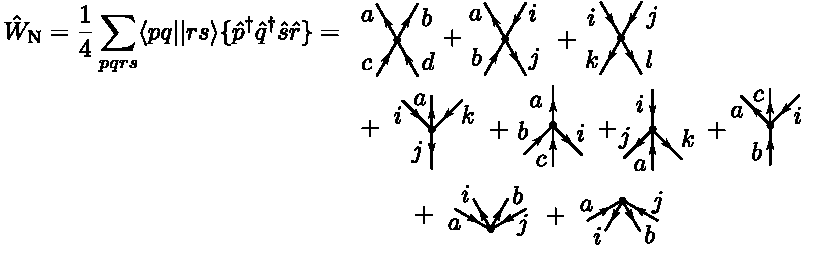
\includegraphics[width=\textwidth]{project2_4b}
\end{centering}That leaves the contributions from the Fock-operator, and that is where the 
three cases will differ. The final term is given by
$$\op{F}_{\rm N} = \sum_{pq} f_{pq} \{\op{p}^\dagger \op{q}\}.$$

For the general case, no terms vanish, so we have

\begin{centering}
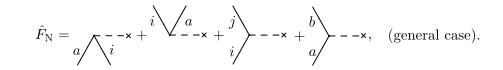
\includegraphics[width=\textwidth]{project2_4c}
\end{centering}

If we have a non-canonical Hartree-Fock case, the first two terms are guaranteed to vanish, as they are contained in the off-diagonal blocks of the Fock-matrix. So we are left with

\begin{centering}
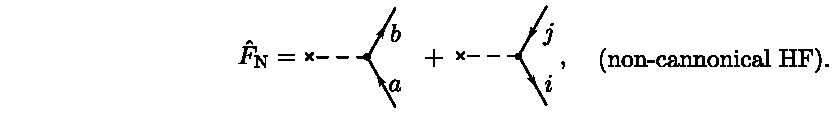
\includegraphics[width=\textwidth]{project2_4d}
\end{centering}

For the cannonical Hartree-Fock case, only the diagonal terms $f_{aa}$ and $f_{ii}$ survive, so we have

\begin{centering}
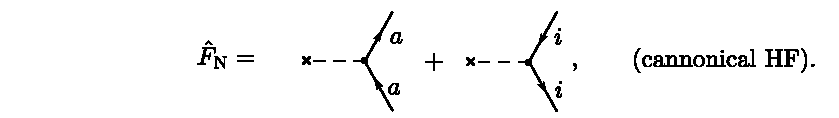
\includegraphics[width=\textwidth]{project2_4e}
\end{centering}

\clearpage

\section*{Exercise 5)}

We will now set up the Hartree-Fock equations. While we will describe briefly how these are found, we won't show the derivation in detail, as this was done in the previous midterm project. For a detailed explanation of the Hartree-Fock equations and their origin, look to exercise 1e in midterm project 1.

\subsubsection*{Setting up the equations}

The first step to finding the Hartree-Fock equations is setting up the reference energy of a general Slater determinant
$$E_{\rm ref} = \braopket{\Phi}{\op{H}}{\Phi} = \sum_{p=1}^N \braopket{p}{\op{h}_0}{p} + \frac{1}{2}\sum_{p=1}^N\sum_{q=1}^N\braket{pq|}{pq}.$$
We then expand the states $p$ into another general basis
$$E = \sum_{p=1}^N \sum_{\alpha \beta} C^*_{p \alpha} C_{p \beta}\braopket{\alpha}{\op{h}_0}{\beta} + \frac{1}{2}\sum_{p=1}^N\sum_{q=1}^N\sum_{\alpha\beta\gamma\delta} C_{p\alpha}^* C_{q \beta}^* C_{p \gamma} C_{q \delta} \braket{\alpha\beta|}{\gamma\delta}.$$
We can now minimize the reference energy with respect to the coefficients $C$. This is a mathematical minimization problem with constraints resulting from limitations in the wavefunctions. Introducing the Lagrangian multipliers $\eps_k$, we get $k$ equations
$$h^{\rm HF} \mathbf{C}_k = \eps_k \mathbf{C}_k.$$
Here $h^{\rm HF}$ is a matrix with elements given by
$$h^{\rm HF}_{\alpha\gamma} = \braopket{\alpha}{\op{h}_0}{\gamma} + \sum_{p=1}^N\sum_{\beta\delta} C_{p\beta}^* C_{p \delta} \braket{\alpha\beta|}{\gamma\delta}.$$

\subsubsection*{Solving the equations}

When solving the Hartree-Fock equations, we usually do it as an iterative process, but as we will see, we don't really have to do any iterations---it turns out we are already in the correct basis! We will now show this. For the first iteration, we start of by claiming $C_{pq} = \delta_{pq}$, this is simply due to the fact that we start in our original basis. 
The elements of $h^{\rm HF}$ then become
$$h^{\rm HF}_{\alpha\gamma} = \braopket{\alpha}{\op{h}_0}{\gamma} + \sum_{p=1}^N\sum_{\beta\delta} \delta_{p\beta} \delta_{p \delta} \braket{\alpha\beta|}{\gamma\delta}.$$
Performing the sums over $\beta$ and $\delta$ simplifies this to
$$h^{\rm HF}_{\alpha\gamma} = \braopket{\alpha}{\op{h}_0}{\gamma} + \sum_{p=1}^N \brakket{\alpha p}{\gamma p}.$$
Here, the sum over $p$ is actually a sum over the particles in our system, thus the sum actually corresponds to a sum over all the hole states of the system. We then recognize that the elements are equal to the Fock-elements we found in the previous exercise
$$h^{\rm HF}_{pq} = f_{pq} = \braopket{p}{\op{h}_0}{q} + \sum_{i} \brakket{pi}{qi}.$$

Let us explicitly calculate these elements. For our system, the one-body operator is given by
$$\op{h}_0 = \sum_{p\sigma} (p-1)\op{a}_{p\sigma}^\dagger \op{a}_{p\sigma}, \quad h_{pq} = \delta_{pq} (p-1),$$
so we immediatly see that the one-body operator is diagonal in the sense $h_{pq} = \delta_{pq} k_p$.

For the two-body operator we have 
$$\op{v} = -\frac{g}{2}\sum_{pq}\op{P}_{p}^+ \op{P}_{q}^-.$$
So we have
$$u_{pq} = -\frac{g}{2} \sum_{i} \brakket{pi}{qi} = \sum_i\sum_{rs} \braopket{pi}{\op{P}_{r}^+ \op{P}_{s}^-}{qi}_{AS},$$
note that in this sums over $p, q$ and $i$ sum over both of the quantum numbers $p$ and $\sigma$, but the sums over $r$ and $s$ only sum over the first quantum number.

If we let a bar denote the same state, but with opposite spin we see that for $\op{P}^-_s\ket{q i}$ to 
not vanish, we must have $i=\bar{q}$. An
d for $\bra{pi}\op{P}^+_r$ to not vanish, we
 need $i=\bar{p}$. Meaning we only get a contribution to $u_{pq}$ if and only if $p$ and $q$ are the same hole state. We can summarize this result as
\begin{align*}
u_{ap} &= u_{pa} = 0, \\
u_{ij} &= -\delta_{ij} g/2.
\end{align*}


We define our model space to consist of the single-particle levels $p=1,2$ and the excluded space is then $p=3,4$. This means we define our reference state to be
$$\ket{\Phi_0} = \op{P}_1^+ \op{P}_2^+ \ket{0},$$
We can then set up our Hartree-Fock matrix
\begin{align*}
h^{\rm HF} = 
\begin{pmatrix}
-g/2 & 0 & 0 & 0 & \quad 0 & \quad 0 & \quad 0 & \quad 0 \\
0 & -g/2  & 0 & 0 & \quad 0 & \quad 0 & \quad 0 & \quad 0 \\
0 & 0 & 1-g/2 & 0 & \quad 0 & \quad 0 & \quad 0 & \quad 0 \\
0 & 0 & 0 & 1-g/2 & \quad 0 & \quad 0 & \quad 0 & \quad 0 \\
0 & 0 & 0 & 0 & \quad 2 & \quad 0 & \quad 0 & \quad 0 \\
0 & 0 & 0 & 0 & \quad 0 & \quad 2 & \quad 0 & \quad 0 \\
0 & 0 & 0 & 0 & \quad 0 & \quad 0 & \quad 3 & \quad 0 \\
0 & 0 & 0 & 0 & \quad 0 & \quad 0 & \quad 0 & \quad 3 \\
\end{pmatrix}
\end{align*}
And we now see that the matrix is \emph{already diagonal}, so there really isn't anything to solve here. The eigenvalues of the matrix are equal to the diagonal elements, and the eigenvectors are simply the unit vectors: $C_k = \hat{e}_k$. This means we were already in the correct basis, and our Hartree-Fock iteration didn't change our basis.

\subsection*{Finding the reference energy}
We have now shown that our original basis already gave a minimum for the reference energy, so let us calculate this reference energy. As our basis did not change, we can find it from the expression
$$E_{\rm ref} = \braopket{\Phi}{\op{H}}{\Phi} = \sum_{p=1}^N \braopket{p}{\op{h}_0}{p} + \frac{1}{2}\sum_{p=1}^N\sum_{q=1}^N\braket{pq|}{pq}.$$
Again, the sums over $N$ comes from the particles in our system, and so for the ground state, they actually correspond to the hole states, so we have
$$E_{\rm ref} = \braopket{\Phi_0}{\op{H}}{\Phi_0} = \sum_{i} \braopket{i}{\op{h}_0}{i} + \frac{1}{2}\sum_{ij} \brakket{ij}{ij}.$$
The hole states are now $i\in\{1_\u, 1_\d, 2_\u, 2_\d \}$, a quick calculation then gives us the reference energy. For the one-body operator we have
\begin{align*}
\braopket{i}{\op{h}_0}{i} &= (p-1) \quad \Rightarrow \quad \sum_{i} \braopket{i}{\op{h}_0}{i} = 2.
\end{align*}
And for the two-body operator, we see that any matrix elements with broken pairs will vanish, leaving us with
\begin{align*}
E_{\rm ref} &=   
\frac{1}{2}\big(
\brakket{1_\u1_\d}{1_\u1_\d} + \brakket{1_\d1_\u}{1_\d1_\u}
+ \brakket{2_\u2_\d}{2_\u2_\d} + \brakket{2_\d2_\u}{2_\d2_\u}
\big).
\end{align*}
Here, all terms contribute $-g/2$, so we get the final result
$$E_{\rm ref} = 2-g.$$

\subsection*{Finding the correlation energy}

Let us take a quick recap of what we have done so far. In exercise 2 we defined an ansatz ground state and then found the possible 2p2h and 4p4h excitations from this ansatz ground state. This gave us a complete orthogonal basis for our system. With a complete basis, we could represent the Hamiltonian as a matrix and diagonalize it to find the lowest eigenvalue of the Hamiltonian, which by definition is the ground state energy. As we had a complete basis, we knew our result was actually the exact solution for our system. 

In exercise 3 we tried truncating the 4p4h excitation, meaning we no longer had a complete basis. By diagonalizing the Hamiltonian in this incomplete basis, we found a ground state energy, but this time it was an approximate result. Due to the variational principle we expected this aprroximation to lie above the exact result, which it did for $g=0$.

Now, in this exercise, we have looked at the Hartree-Fock method. It is important to remember that the Hartree-Fock method simply finds the single Slater determinant with the lowest energy of the system. There is no guarantee that the ground state energy is actually given by a single Slater determinant, instead it must usually be expressed as a linear combination of different SDs, such as we did in exercise 2 and 3. The Hartree-Fock method therefore doesn't find the exact energy, and it doesn't really aim to do that at all---it simply finds the reference energy.

Now, this means that we have the exact solution, which is given by a combination of different SDs, and we have the reference energy, the best single SD energy. The difference between these two energies is known as the correleation energy, so we have
$$E_{\rm exact} = E_{\rm correlation} + E_{\rm ref}.$$
As we know the exact energy from exercise 2, and found the reference energy in this exercise, we can easily compute the correlation energy as a function of $g$. The results of these calculations is shown in figure \ref{fig:correlation_energy}.

\begin{figure}[htbp]
\centering 
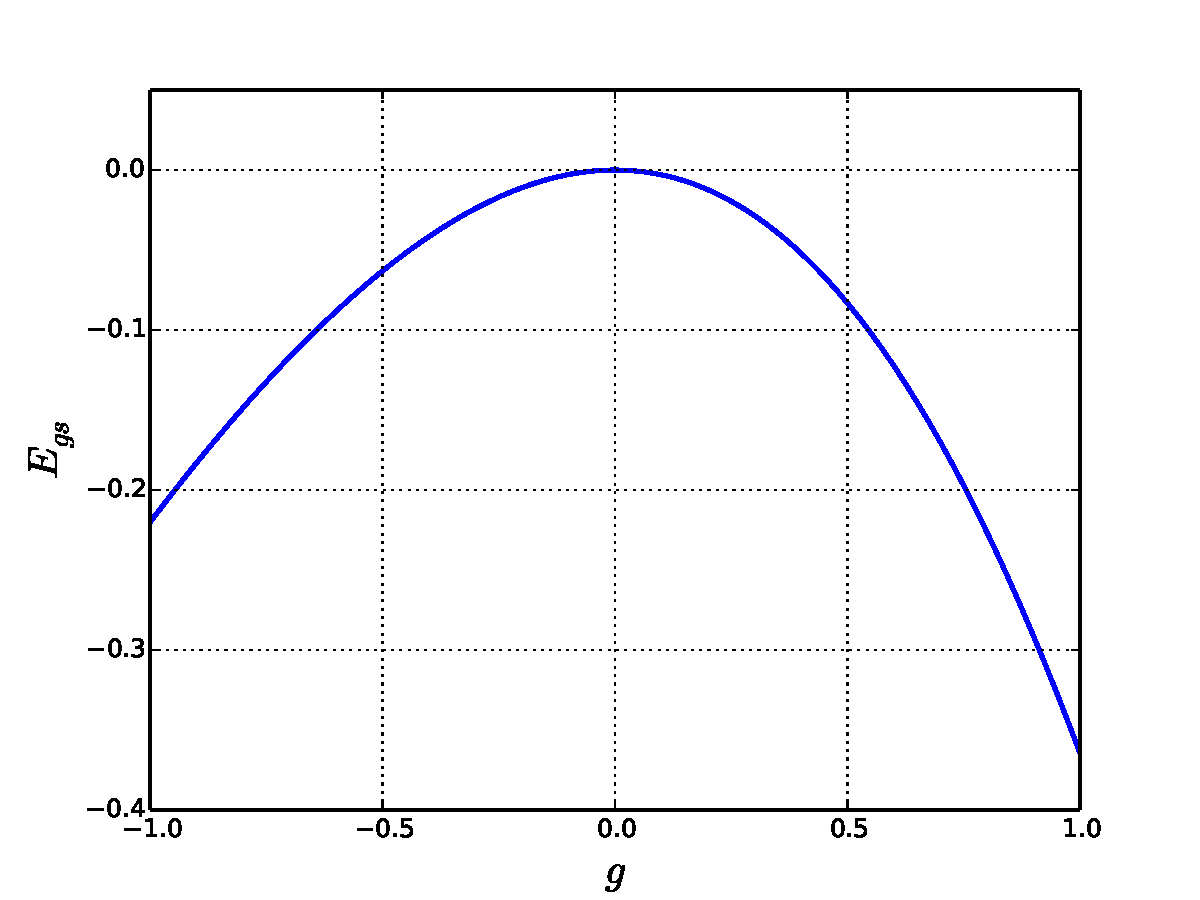
\includegraphics[width=0.8\textwidth]{proj2_correlation}
\caption{The correlation energy of the system as a function of the interaction strength. \label{fig:correlation_energy}}
\end{figure}

Note that the correlation energy is only $0$ for $g=0$. This means that only the case where there is no interaction has a ground state that can be described by a single Slater determinant.

\subsection*{Perturbation theory}

We just saw how the Hartree-Fock method gave us the reference energy. Now we want to find some approximate method that can give us the \emph{correlation energy}. To do that, we turn to many-body perturbation theory. The basis for this method is quite elaborate, so we won't go into details now, but they can be found in for example Shavitt and Bartlett.

In exercise 4, we split the Hamiltonian into the reference energy, the Fock-operator and the term we called the perturbation term
$$W_{\rm N} = \frac{1}{4}\sum_{pqrs} \brakket{pq}{rs} \{\op{p}^\dagger\op{q}^\dagger\op{s}\op{r}\}.$$
And it is this term we now look at. However, as mentioned in exercise 4, as long as we do not have a cannonical HF case, we will also add the $F^{\rm o}$ term to the perturbation, which is the off-diagonal elements of the Fock-operator.

We now look at perturbation to the third order. The zero and first order combined simply gives us the reference energy, and as we are interested in the correlation energy, we look at the second and third orders only. All possible second and third order contributions are shown in figure 2 in the exercises. We will now discuss which of these diagrams are important in our case. Let us start by looking in detail and 1 and 2, simply to see the system of the diagrams, and then we will go through the rest of the diagrams a bit faster.

Diagrams 1 and 2 are the only two diagrams that form the second order contribution. All the diagrams are drawn as anti-symmetric Goldstone diagrams, and we must remember to include a Resolvent line between any vertical set of operators, even tough they are not drawn in. Looking at diagram 1, we can interpret this diagram as
\begin{align*}
  \mbox{(diag.\ 1)} = \frac{1}{4}\sum_{abij}\frac{\brakket{ab}{ij}\brakket{ij}{ab}}{\eps_{ij}^{ab}}.
\end{align*}
Here, the matrix elements in the denominator are found from the two-body operator at the top and bottom, as we are looking at the product, the order is unimportant. The numerator is given by the resolvant line, and is given by what hole lines and particle lines cross the resolvant line. The term $\eps_{ij}^{ab}$ should be interpred as
$$\eps_{ij}^{ab} = \eps_i + \eps_j - \eps_a - \eps_b.$$
The sums over $a,b,i$ and $j$ are implicit as we have two hole and two particle lines. Finally, the $1/4$ weight-factor is added because the two particle and two hole lines are both equivalent, so each pair adds a factor of $1/2$.

Similarily for figure 2, remembering the resolvant line, we get
\begin{align*}
  \mbox{(diag.\ 2)} = \sum_{ai}\frac{\braopket{a}{\op{f}}{i}\braopket{i}{\op{f}}{a}}{\eps_{i}^a}.
\end{align*}
This time we only get a sum over $a$ and $i$ as we have a single particle and single hole line. No equivalent lines means to extra weight factors. The resolvent in the denominator becomes $\eps_i^a = \eps_i - \eps_a$ as it is only crossed by two lines. The denominator is given by the two one-body matrix elements, the order is unimportant. This figures shows and important result, as figure 2 has both $f_{ai}$ and $f_{ia}$ in the denominator, it vanishes for a Hartree-Fock basis---figure 2 only has to be included in the general case.

The interpretations of the third order figures is completely analogous. The main difference is that since there's three operatos working, the denominator will in each case consist of the product of three matrix elements and the numerator will be the product of two resolvant contributions. Let us look at diagram 4 as an example, it becomes
\begin{align*}
  \mbox{(diag.\ 4)} = \frac{1}{8}\sum_{abcdij}\frac{\brakket{ab}{ij}\brakket{ab}{cd}\brakket{cd}{ij}}{\eps_{ij}^{ab}\eps_{ij}^{cd}}.
\end{align*}

Now that we have looked at some examples, we noted that figure 2 vanishes for the Hartree-Fock case. Looking at the third-order diagrams, we recognize that diagrams 6, 7, 10, 11, 12, 13, 14, 15 and 16 all vanish in the HF case as they are multiplied with at least one $f_{ai}$ matrix element. Note that diagrams 8 and 9 do \emph{not} necessarily vanish in the HF-case, as they only have $f_{ab}$ and $f_{ij}$ elements, which are non-zero in the non-cannonical cases. At first glance, one might consider the diagram to contribute  in the cannonical term as well, but we have to remember that it is only the off-diagonal part of the Fock-operator that contributes in the perturbation, so the diagrams do in fact vanish for the cannonical case.

\clearpage

In sumamry, we have seen that diagrams 1, 4 and 5 contribute to both the cannonical and the non-cannonical HF cases, while diagrams 8 and 9 only contribute in the non-cannonical
\begin{center}
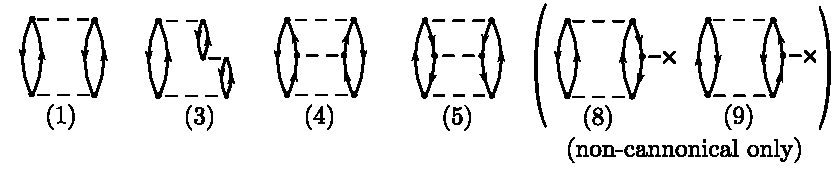
\includegraphics[width=\textwidth]{project2_5}
\end{center}

Now, the discussion of the diagrams so far has not used any information about our specific interaction, and the results so far are valid for any interaction. Now however, we will use our knowledge of our interaction to simplify things even further.

If we write out diagram three, we see that it has the form
\begin{align*}
    \mbox{(diag.\ 3)} = \sum_{abcijk}\frac{\brakket{ij}{ab}\brakket{ac}{jk}\brakket{bk}{ci}}{\eps_{ij}^{ab}\eps_{kj}^{ac}}.
\end{align*}
Our interaction only acts between pairs of particles with the same quantum number $p$. If we then look at the matrix element $\brakket{bk}{ci}$, we see that this element must be zero, as $b$ is a particle state and $k$ is a hole state, so $\brakket{bk}{ci} = 0$ and so diagram 3 vanishes as a result of the nature of the interaction.

In the cannonical Hartree-Fock case, there is then only three contributing diagrams, which are
\begin{align*}
    \mbox{(diag.\ 1)} &= \frac{1}{4}\sum_{abij}\frac{\brakket{ab}{ij}\brakket{ij}{ab}}{\eps_{ij}^{ab}}, \\
    \mbox{(diag.\ 4)} &= \frac{1}{8}\sum_{abcdij}\frac{\brakket{ab}{ij}\brakket{ab}{cd}\brakket{cd}{ij}}{\eps_{ij}^{ab}\eps_{ij}^{cd}},\\
    \mbox{(diag.\ 5)} &= \frac{1}{8}\sum_{abijkl}\frac{\brakket{ab}{ij}\brakket{kl}{ij}\brakket{ab}{kl}}{\eps_{ij}^{ab}\eps_{kl}^{ab}}.
\end{align*}

Summing all these contributions by hand is pretty tedious work, but we can easily do them through a simple python script. We can then plot the correlation energy found both from only the second order contribution (digram 1) and up to third order (diagrams 1, 4 and 5). The results is shown in the following figure.

We see that the approximation to both second and third order are very good when the interaction is weaker $g\in[-0.5,0.5]$, but as the interaction gets stronger the approximation becomes worse. We also note that the third-order is actually worse than the second order for a strong interaction! This result illuminates the difference between perturbation theory and configuration interaction we noted earlier, including higher-order terms can \emph{possibly give a worse result} for perturbation theory---for CI however, including more excitations will never give a worse result. We also see the consequences of perturbation theory not being a variational method, as both approximations undershoot the true ground state correlation energy of the system.



\begin{figure}[htbp]
\centering
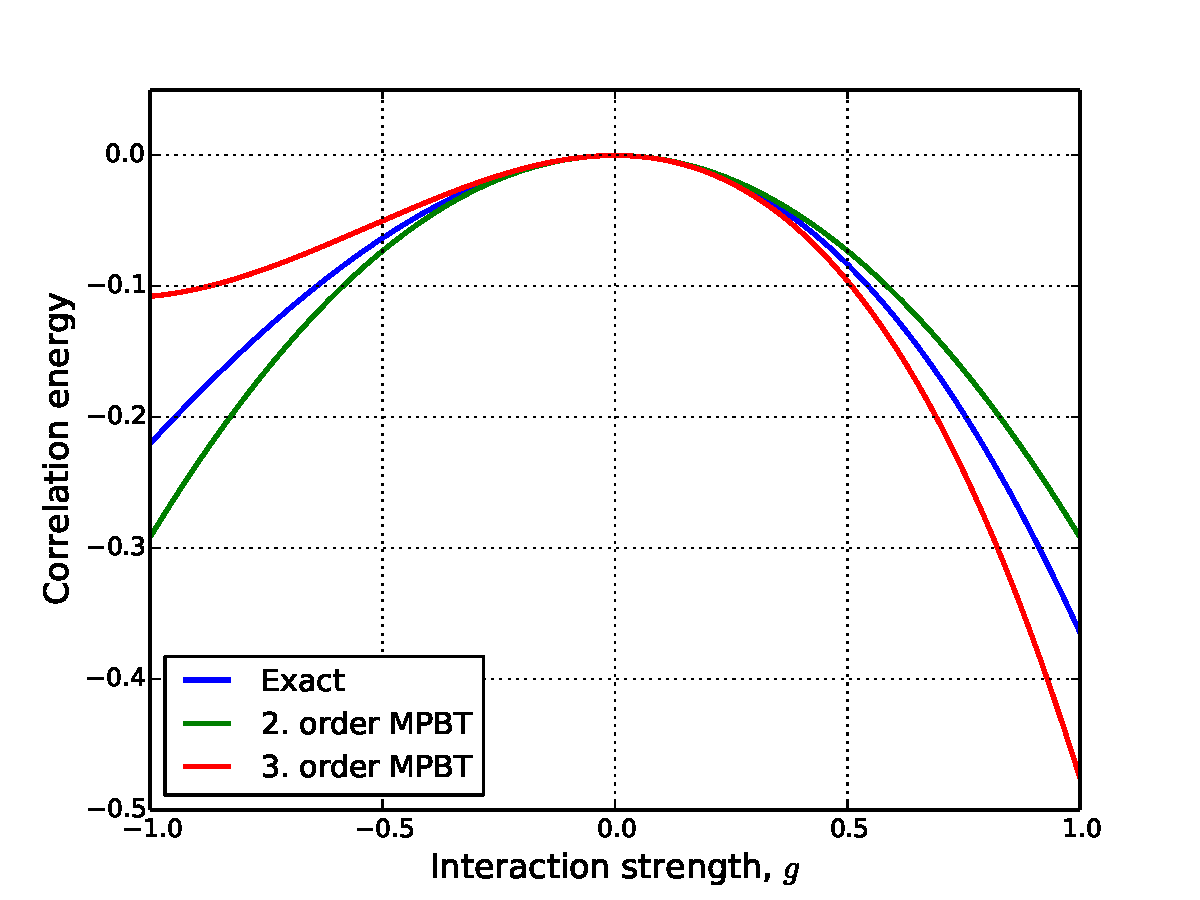
\includegraphics[width=\textwidth]{pert_1.pdf}
\caption{The energy contribution from MBPT up to second and third order.}
\end{figure}


\clearpage

\section*{Exercise 6}

Now, we have looked at how perturbation theory approximates the correlation energy, and how this approximation behaves compared to the CI-case. Now let us look at how perturbation theory approximates the ground state of the system. For the CI-case we found the coefficients of all 2p2h SDs, so let us find these coefficients to second order with MBPT. To get from the reference state to the perturbed wave-function, we have to turn to the \emph{wave operator}, $\Omega$.

If we let $\ket{\Psi^{(1)}_0}$ denote the perturbed wave function, and $\ket{\Phi_0}$ our reference state, we know that we have
$$\ket{\Psi^{(1)}_0} = (1 + \Omega^{(1)})\ket{\Phi_0}.$$
This means $\Omega^{(1)}\ket{\Phi_0}$ is the the correction term in the wave function from the reference state. The wave-operator for the second-order perturbed wave function is given by\footnote{See Shavitt and Bartlett section 2.4.7, p. 43.}
$$\Omega^{(1)} = \op{R}_0 \op{V}.$$
Which gives
\begin{align*}
\ket{\Psi^{(1)}_0} - \ket{\Phi_0} &= \op{R}_0 \op{V}\ket{\Phi_0} \\
&= \frac{1}{4}\sum_{ai} \frac{\brakket{a\bar{a}}{i\bar{i}}}{\eps_{ii}^{aa}}\ket{\Phi_{i}^{a}}.
\end{align*}
So we can write the perturbed wave-function as
$$\ket{\Psi^{(1)}_0} = \ket{\Phi_0} + \frac{1}{4}\sum_{ai} \frac{\brakket{a\bar{a}}{i\bar{i}}}{\eps_{ii}^{aa}}\ket{\Phi_{i}^{a}}.$$
However, we know that we can expand any wave-function describing our system into the SD-basis we used in exercise 3. We get
$$\ket{\Psi^{(1)}_0} = C_0\ket{\Phi_0} + C_2^3\ket{\Phi_2^3} + C_2^4\ket{\Phi_2^4} + C_1^3\ket{\Phi_1^3} + C_1^4\ket{\Phi_1^4}.$$
By comparing these two expressions we can find the coefficients for the perturbed wave function. We get
\begin{align*}
C_2^3 = -\frac{g}{16}, \qquad C_2^4 = -\frac{g}{32}, \qquad C_1^3 = -\frac{g}{32}, \qquad C_1^4 = -\frac{g}{64}.
\end{align*}
An important issue here is that $C_0 = 1$, and so the perturbed wave function is \emph{not normalized}. This is because perturbation theory is formulated with what is known as \emph{intermediate} normalization. This is rather trivial to solve, we simply divide all coefficients by the normalization-factor $\sqrt{\sum_i |c_i|^2}$.

To compare with the approximation from CI, let us compute the coefficients for $g=1/2$, we get the coefficients
\begin{align*}
C_0 &= 0.997, \quad C_2^3 = -0.062,  \quad C_2^4 = -0.031, \quad C_1^3 &= -0.031, \quad C_1^5 = -0.016.
\end{align*}

Compared to the CI results, we see that the reference state plays a much bigger part of the perturbed wave function. This is not a surprise, as CI adds the 2p2h excitations to infinite order, and we have now only included the 2p2h excitations to first order, higher order of 2p2h excitations will cause more of the wave-function to move out of the reference state and into the 2p2h excited states.


\clearpage

\section*{Exercise 7}

We now turn to MBPT to the fourth order. We now get a lot of diagrams that can contribute to the energy, so we limit our discussion to the cannonical HF-case only. All of the diagrams in the cannonical case are shown in figures 3, 4, 5 and 6 of the exercises. Just like before, these are completely general diagrams, and we will show that we can disregard quite a lot of them. First we look at the linked-diagram theory, then we look closer at the diagrams. 

A diagram is called unlinked if and only if it has a disconnected part that is closed, meaning it has no open lines. Goldstones linked-diagram theorem states that all unliked diagrams will cancel agains the renormalization terms in RSPT, meaning we can express the energy and wave function in each order as a sum of linked diagrams only\footnote{See Shavitt and Bartlet section 5.8.}. This means we can immediately disregard diagram 33 and 41.

Let us now go through all the diagrams and find those that vanish due to having broken pairs, i.e., the diagrams that vanish due to our specific interaction. Take for example diagram 1, which vanishes due to having a term $\brakket{ab}{ci}$. From this argument, we see that all four diagrams from figure 3 vanish. Let us illustrate this by drawing red circles around all the matrix elements that are zero in figure 3.

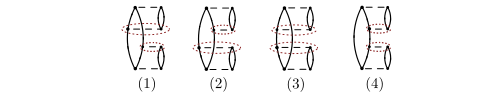
\includegraphics[width=\textwidth]{project2_6}

Without taking the time to draw up all the diagrams, the same arguments shows that most diagrams in figure 4 also dissapear. Going through all the diagrams, we see that 5, 6, 14 and 15 are the ones that do not vanish for figure 4. For figure 5 we actually see that all diagrams vanish again. For figure 6 we already found that 33 and 41 vanished due to being unlinked---the rest contribute to the perturbation.

All diagrams for figure 3 and 5 vanished for our interaction, this is definitly not a surprise, as those figures correspond to 1p1h and 3p3h excitations respectively. As our reference state already has the four particles positioned in two pairs, it goes without saying that and odd number of particle excitations neccesitates broken pairs and will vanish. The same argument also explained why there were no diagrams that vanished for figure 6. That figure shows the four-particle-four hole excited states, but as we only have four particles in our system, exciting all the particles will keep them collected in pairs, so we get no ubroken pairs. For the diagrams in figure 4 however, we have 2p2h excitations, and so the diagrams that vanish correspond the the cases where we excite one particle from either pair, or excite both particles in one pair, but into different levels, leaving us with a broken pair.

\clearpage

We are now ready to calculate the contribution from the diagrams that do not vanish. These are our diagrams

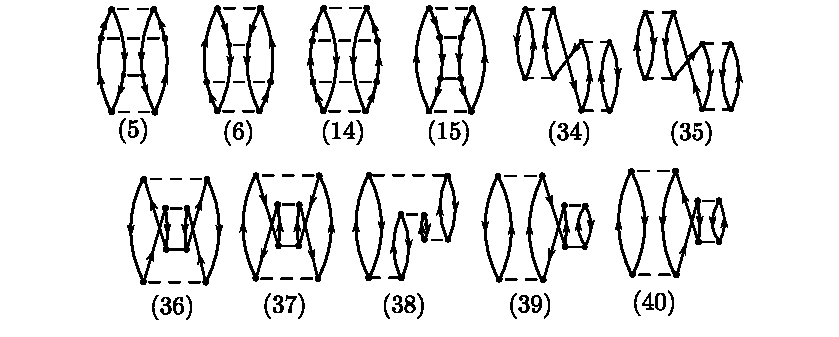
\includegraphics[width=\textwidth]{project2_7}

We would now like to express all these diagrams algebraicly, luckily, diagrams 5 and 6, 14 and 15, 34 and 35, 36 and 37 and 39 and 40 are all conjugate diagrams of each other, meaning they contribute the same algebraic expression. So we only need to set up the following expressions

Algebraicly, we can express these contributions as follows
\begin{align*}
\mbox{(diag.\ 5)} &= \frac{1}{16}\sum_{\substack{abcd \\ ijkl}} 
\frac{\brakket{ij}{ab}\brakket{ab}{cd}\brakket{kl}{ij}\brakket{cd}{kl}}{\eps_{ij}^{ab}\eps_{ij}^{cd}\eps_{kl}^{cd}}, \\[0.2cm]
%
%
\mbox{(diag.\ 14)} &= \frac{1}{16}\sum_{\substack{abcdef \\ ij}} 
\frac{\brakket{ij}{ab}\brakket{ab}{cd}\brakket{cd}{ef}\brakket{ef}{ij}}{\eps_{ij}^{ab}\eps_{ij}^{cd}\eps_{ij}^{ef}}, \\[0.2cm]
%
%
\mbox{(diag.\ 34)} &= -\frac{1}{4}\sum_{\substack{abcd \\ ijkl}} 
\frac{\brakket{ij}{ab}\brakket{ab}{ik}\brakket{kl}{cd}\brakket{cd}{kl}}
{\eps_{ij}^{ab}\eps_{ijkl}^{abcd}\eps_{jl}^{cd}}, \\[0.2cm]
%
%
\mbox{(diag.\ 36)} &= \frac{1}{16}\sum_{\substack{abcd \\ ijkl}} 
\frac{\brakket{ij}{ab}\brakket{kl}{cd}\brakket{ab}{kl}\brakket{cd}{ij}}
{\eps_{ij}^{ab}\eps_{ijkl}^{abcd}\eps_{ij}^{cd}}, \\[0.2cm]
%
%
\mbox{(diag.\ 38)} &= \sum_{\substack{abcd \\ ijkl}} 
\frac{\brakket{il}{ad}\brakket{jk}{bc}\brakket{cd}{kl}\brakket{ab}{ij}}
{\eps_{il}^{ab}\eps_{ijkl}^{abcd}\eps_{ij}^{ab}}, \\[0.2cm]
%
%
\mbox{(diag.\ 39)} &= -\frac{1}{4}\sum_{\substack{abcd \\ ijkl}} 
\frac{\brakket{ij}{ab}\brakket{kl}{cd}\brakket{cd}{kl}\brakket{ab}{ik}}
{\eps_{ij}^{ab}\eps_{ijkl}^{abcd}\eps_{ik}^{ab}}.
\end{align*}

As before, calculating all these sums is very tedious, luckily, a few lines of python code solves them for us. On the next page we give a plot of the the result of the approximation energy up to the fourth order MBPT. As we won't go any further than fourth order in this project, we also make a log-plot of the error in each approximation to the correlation energy.


\begin{figure}[p]
\centering
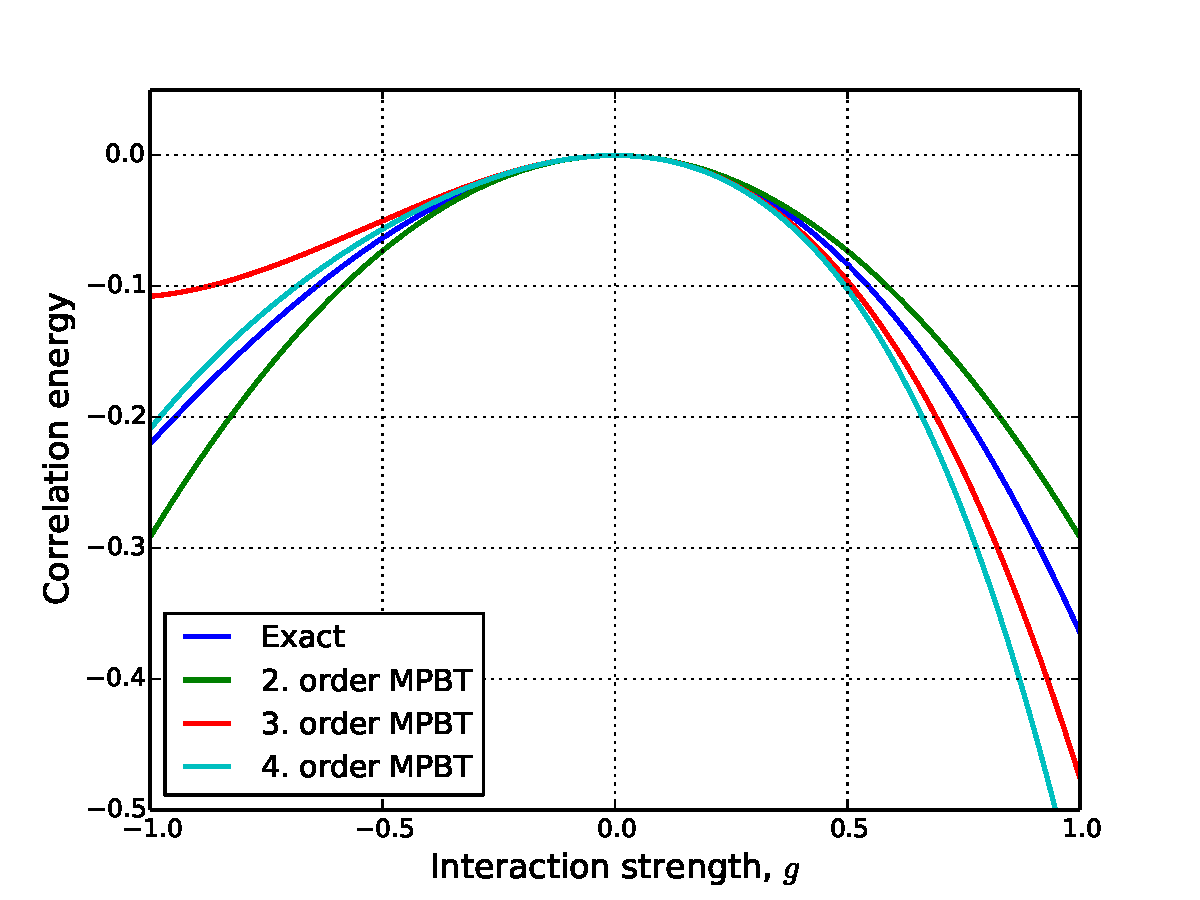
\includegraphics[width=\textwidth]{pert_2.pdf}
\caption{Correlation energy up to fourth order MBPT.}
\end{figure}

\begin{figure}[p]
\centering
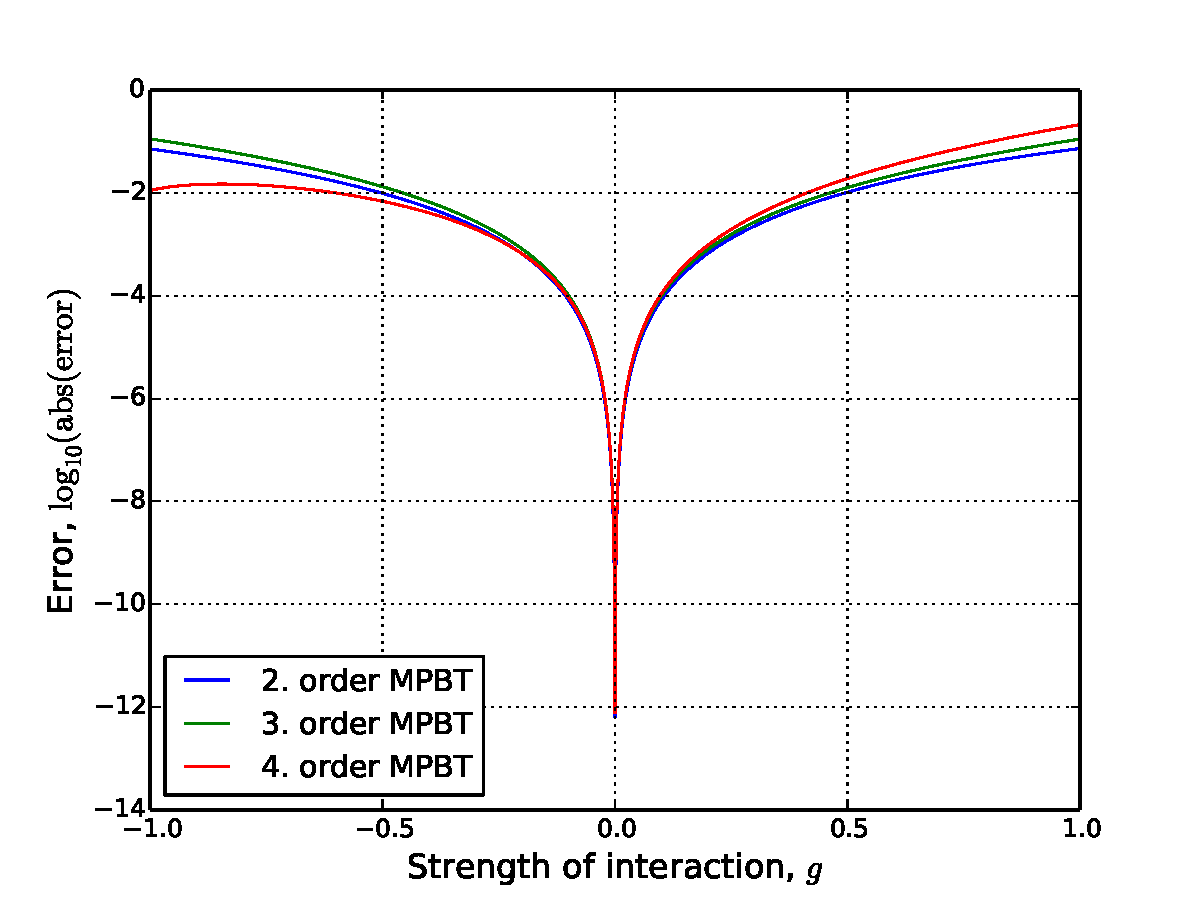
\includegraphics[width=\textwidth]{logerror.pdf}
\caption{Error in the approximation to the correlation energy up to fourth order MBPT.}
\end{figure}

\clearpage

From the figures, we see that the fourth order MBPT approximation to the correlation energy is better than the lower orders for $g<0$, but worse than the lower orders for $g>0$. Again this shows us an the important point of MBPT---there is no guarantee that the approximation will converge to the exact solution as we increase the order. In fact, as we see in our case, increasing the order of the approximation might actually give you a worse result! Also, we see that MBPT is not variational, so we can't simply calculate the approximation of many different orders and choose the smallest one, as we then run the risk of undershooting the real ground state energy.

\section*{Summary}

In this project we started out by defining a very simple system. We showed that the Hamiltonian commuted with the spin project operators and forced a total spin of $S=0$, which is then a conserved qunatity in the interaction. From this we noted that it would be practical to define our interaction in terms of pair creation and annihilation operators.

As our system only has a finite number of states, we were able to perform a full configuration interaction calculation on it, and we therefore got the exact ground state of the system. Normally, one cannot do a FCI calculation of a system, as there are infinite possible excited states, and so one must truncate the excitations somewhere, this leads to a non-complete configuration interaction calculation.

To compare a full and an incomplete CI, we limited our system to 2-particle 2-hole excitations, this mean cutting out one of the six Slater determinants that comprised our basis. It turned out that the CI from this truncated and incomplete basis was still really good, which was not strange as the 4p4h contribution was not really important for the ground state of the system.

Next we turned to the Hartree-Fock method, which normally is used as a starting point, as it lets us find a basis where we can define our reference state to have the lowest possible energy, i.e., find the single Slater determinant with the lowest possible energy of the system. It turned out that the Hartree-Fock matrix was diagonal, meaning our basis was already the best basis for a reference state. This meant that the reference state we defined in exercise 2 is the single Slater determinant with the lowest energy of the sytem, and we calculated the reference energy from this SD. 





\end{document}
